\documentclass[a4paper, 10pt]{iopart}
\usepackage{graphicx}
\usepackage{harvard}

\begin{document}

\title[A novel approach to model program functions relationship]{A
  novel approach to model the network of program functions in the
  Linux operating system}

\author{A S Rock$^1$, O J Dahl$^2$}
\address{$^1$ Open Faculty, Azteria}
\address{$^2$ Union University, Teoplia}
\ead{rock@open.edu}
\date{\today}

\begin{abstract}
We constructed a graph from linux kernel functions relationship and
discovered power law behaviour of outdegree distribution.
\end{abstract}

\noindent{\it Keywords\/}: graph, complex network, linux kernel.

\submitto{\NJP}
\maketitle

\section{Introduction}

In a previous work, we propose a statistical and complex network
approaches to model culinary diversity and evolution in the
relationship between recipes and ingredients of four different cookery
books~\cite{culinary:njp:2008}. In this work, we use the same approach
to model static relationship of functions using an operating system
source code as input data.

\section{Graph construction}

We constructed a $G$ graph with the following convention: 
the functions are the vertices and the arcs come from the callee
function to the caller function as showed in the Figure~\ref{fig:fungraph}.

\begin{figure}[ht]
  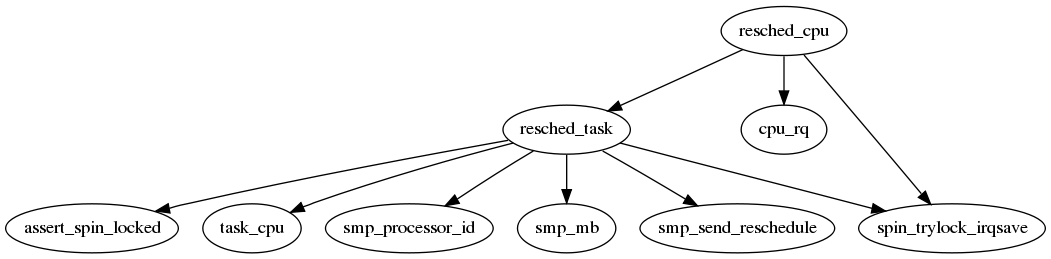
\includegraphics[width=0.9\textwidth]{img/fungraph.png}
  \label{fig:fungraph}
  \caption{Directed subgraph of functions {\tt resched\_task} and {\tt
      resched\_cpu} of the linux kernel scheduler.}
\end{figure}

\section{Results}
The Figure~\ref{fig:outdegree} shows the cumulative distribution of
the outdegree values.

\begin{figure}[ht]
  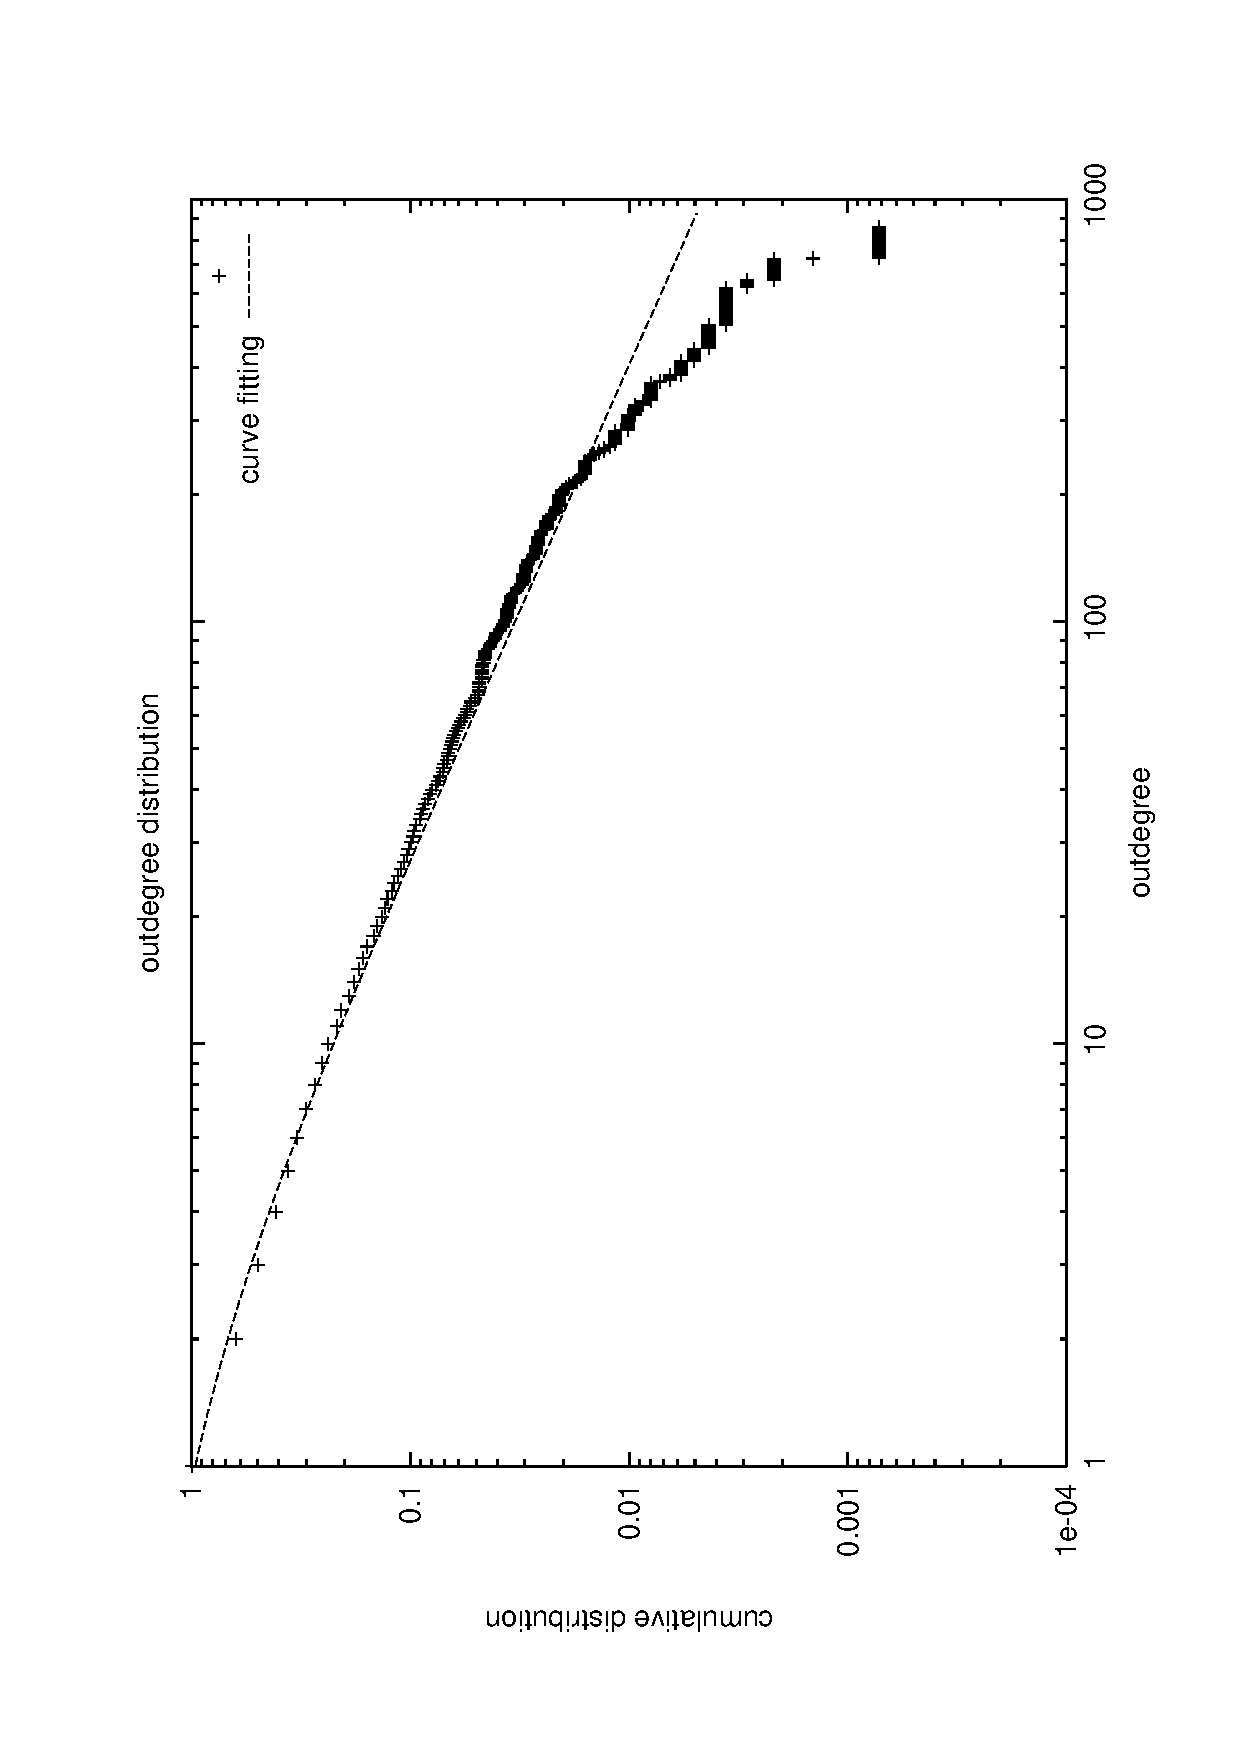
\includegraphics[width=0.75\textwidth]{img/curve}
  \label{fig:outdegree}
  \caption{Outdegree distribution of linux kernel functions.}
\end{figure}

% thanx
\ack{We would like to acknowledge J Silva for the fruitful discussions.}

\section*{References}
%\bibliographystyle{acm}	% Association for Computer Machinery 
%\bibliographystyle{vancouver}	% (uses file "vancouver.bst")
\bibliographystyle{kluwer}	% Harvard-like style
\bibliography{myrefs}		% expects file "myrefs.bib"

\end{document}
